\documentclass[times, utf8, seminar]{fer}
\usepackage{booktabs}

% TODO:
% Odredivanje cijena opcija monte carlo simulacijama
    % https://www.youtube.com/watch?v=r67_YRtYcR8
% Implied volatility preko opcija

% Multi-assset VaR
    % https://www.youtube.com/watch?v=zrqI-NbZSj0&t=21s
% ostali todo-ovi
% popravi BS model poglavlje pri kraju - izvod formule

\begin{document}

\title{Stohastičko modeliranje u financijama}

\author{Ivan Almer}

\voditelj{Tomislav Burić}

\maketitle

\tableofcontents

\chapter{Uvod}
Naivno je misliti da se tržište uglavnom ponaša po nekom skupu pravila i da je moguće predvidjeti kretanja s apsolutnom preciznošću. To bi značilo da postoji „besplatan ručak“ i da možemo uvišestručiti naša sredstva bez imalo rizika. Naravno da nitko od nas nije prvi koji se sjetio povećati svoj kapital brzo i efikasno, ali naravno da to ne dolazi bez određene opasnosti da ćemo izgubiti svoj kapital.

Tržište je mjesto sa izuzetno puno igrača gdje svaki igrač želi zaradu i naravno da nitko ne želi gubiti. Kada netko gubi novac, druga ga strana dobiva, ali za svakog igrača u toj velikoj igri gubici su neizbježni. Cilj je što manje puta izvući deblji kraj i što manje biti na gubitničkoj strani.

Svatko može naslijepo uložiti dio svog kapitala u neki financijski instrument i nadati se da će baš na taj način zaraditi, no malo je vjerojatno da će takav potez donijeti puno dobroga. Sigurno postoje i neki bolji načini kako da analiziramo i kvantificiramo kvalitetu naših ulagačkih ideja s ciljem maksimizacije profita. Budući da se tržište ponaša prilično nedeterministički jasno nam je da to neće biti lak zadatak. Upravo s tom idejom dolazimo to toga da se i u naše modele uvede već spomenuti nedeterminizam s određenim karakteristikama i da na taj način pokušamo naučiti promatrati naizgled kaotično ponašanje tržišta.

Stohastički procesi imaju široku primjenu u financijama. Od modeliranja cijena dionica, kamatnih stopa, do određivanja cijena nekih financijskih derivata i procjene rizika ulaganja. Stohastičko modeliranje je oblik financijskog modeliranja koji se koristi za pomoć u donošenju odluka o ulaganju. Takvim pristupom možemo dobiti podatke i predvidjeti moguće ishode s mjerom nepredvidivosti ili slučajnosti. Mnoge firme koriste stohastičko modeliranje da bi optimizirale svoje portfelje i upravljale svojom imovinom. Jedan je od primjera stohastičkog modeliranja, na primjer, Monte Carlo simulacija, kojom se može modelirati ponašanje portfelja temeljeno na razdiobi povrata individualnih dionica.

Svrha ovog seminarskog rada je napraviti pregled i pobliže objasniti načine uporabe stohastičkog modeliranja u financijama. Iza većine modela stoje neke pretpostavke o ponašanju pojava koje promatramo, koje mogu biti opravdane, ali ponekad se ne obraća puno pažnje na te pretpostavke i model se primjenjuje kada to uistinu ne bi trebalo. U tom svjetlu, ovim radom također želim istaknuti i važnost pretpostavki modela i metoda koje će biti opisane.

\chapter{Black-Scholes Model}

Jedan od najpoznatijih modela za određivanje cijena opcija je Black-Scholes model za koji su znanstvenici osvojili Nobelovu nagradu za ekonomiju. Danas se smatra jednim od najboljih načina za određivanje „fer“ cijene opcija, jer bi u protivnom postojala mogućnost arbitraže.

Black-Scholes model ima pretpostavku na distribuciju cijene dionice da ona mora biti log-normalna, što ima smisla jer cijene dionica ne mogu biti negativne. Razlog za korištenje upravo te distribucije je taj da se cijena dionica vrlo često ponaša kao desno nakrivljena distribucija sa nešto debljim repovima.

\begin{figure}[h!]
\centering
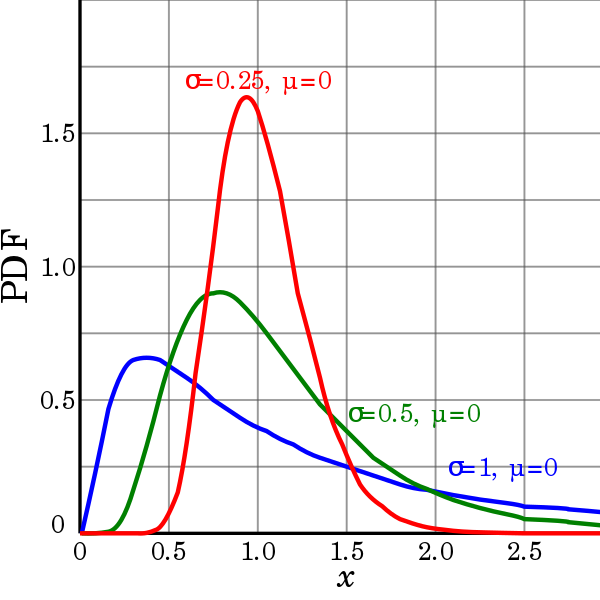
\includegraphics[scale=0.4]{img/log_normal_pdf.png}
\caption{Funkcija gustoće vjerojatnosti log-normalne razdiobe}
\label{fig:log_normal_pdf}
\end{figure}

\noindent Ostale pretpostavke uključuju:
\begin{itemize}
    \item[\textbullet] Opcija je europska (ne može se iskoristiti prije dospijeća)
    \item[\textbullet] Kamatna stopa nerizičnog ulaganja i volatilnost su konstantni
    \item[\textbullet] Dionica ne isplaćuje dividende
    \item[\textbullet] Kretanje tržišta se ne može predvidjeti
\end{itemize}

Izvod ovog modela je mjesto gdje se događaju najzanimljivije stvari i gdje se zapravo najbolje vidi moć stohastičkih procesa. Prvi korak u izvodu je korištenje Itove leme na funkciju cijene opcije za koju vrijedi pretpostavka da ovisi o vremenu i cijeni dionice.

Cijena dionice je modelirana geometrijskim Brownovim gibanjem, a za neki stohastički proces kažemo da ima geometrijsko Brownovo gibanje, ako zadovoljava diferencijalnu jednadžbu:

\begin{centering}
    $dS_t = \mu S_t dt + \sigma S_t dW_t$ \\
\end{centering}

\noindent gdje je $W_t$ Brownovo gibanje definirano kao:
\begin{enumerate}
    \item $W_0 = 0$
    \item $W$ ima nezavisne priraste za svaki $t > 0$
    \item $W_{t+u} - W_t \sim N(0, u)$
    \item $W_t$ je kontinuirano u vremenu
\end{enumerate}

\section{Call i Put opcije}
Opcija je oblik financijskog derivata, koji kupcu ugovora daje pravo, ali ne i obavezu, da pri isteku ugovora (dospijeću) kupi ili proda neko sredstvo po unaprijed dogovorenoj cijeni. Dvije su vrste opcija - call i put. Call opcija kupcu ugovora daje pravo da pri dospijeću kupi sredstvo (npr. dionicu) po cijeni dogovorenoj pri kupnji ugovora. Put opcija se ponaša obrnuto, odnosno kupcu ugovora daje pravo da pri dospijeću proda određeno sredstvo po unaprijed dogovorenoj cijeni. Svaki takav ugovor karakteriziran je sljedećim parametrima:
\begin{itemize}
    \item[\textbullet] cijena ugovora
    \item[\textbullet] dospijeće (vrijeme isteka ugovora)
    \item[\textbullet] izvršna cijena
\end{itemize}

\noindent Primjer uporabe opcija:

Pretpostavimo da možemo trgovati dionicom \textbf{XYZ} kojoj je trenutna cijena $S_0 = 100$. U ovom trenutku mi smo uvjereni da će cijena dionice u budućnosti rasti i kao alternativu direktne kupovine dionice, odlučili smo kupiti call opciju za tu dionicu. Recimo da se $1$ call opcija, izvršne cijene $K = 102$ i dospijeća od jednog mjeseca, prodaje po cijeni $C = 6$, a budući da je jedan ugovor call opcije obično ne odnose na $1$ dionicu nego na njih $100$, onda je cijena jednog takvog ugovora $100 * 6 = 600$. Nakon mjesec dana pogledajmo sljedeća $2$ scenarija:
\begin{itemize}
    \item[\textbullet] cijena dionice se ponaša u skladu s našim očekivanjem i porasla je na $S_t = 120$
    \item[\textbullet] cijena dionice je pala i sada iznosi $S_t = 90$
\end{itemize}
\noindent U drugom slučaju naš ugovor postaje bezvrijedan i gubimo naš uloženi kapital (odnosno naš profit je $-600$). Međutim, u slučaju da se ostvari prvi scenarij možemo iskoristiti pravo da kupimo $100$ dionica po cijeni od $102$. Budući da se te dionice trenutno prodaju po cijeni $120$, nakon što ih kupimo po cijeni od $102$ prodamo ih po tržišnoj cijeni i ostvarili smo profit od $(120 - 102) * 100 - 600 = 1200$.

\section{Pregled formule}

\[ C = N(d_1)S_0 - N(d_2)Ke^{-rt} \]
\[ gdje \hspace{0.1cm} je \hspace{0.2cm} d_1 = \frac{ln\frac{S_t}{K} + (r+\frac{\sigma^2}{2})t}{\sigma\sqrt{t}} \]
\[i \hspace{0.2cm} d_2 = d_1 - \sigma \sqrt{t}\]

\noindent $C =$ cijena Call opcije \\
$N =$ funkcija razdiobe normalne razdiobe\\
$S_0 =$ trenutna cijena dionice (spot price)\\
$K =$ izvršna cijena dionice (strike price)\\
$r =$ kamatna stopa nerizičnog ulaganja\\
$t =$ vrijeme do dospijeća\\
$\sigma =$ volatilnost cijene dionice \\

\noindent Kada imamo sve gore navedene parametre, formulom dobijemo cijenu europske call opcije. Cijena put opcije iste dionice, s istim dospijećem i istom izvršnom cijenom dobije se pomoću put-call pariteta koji povezuje te dvije cijene:

    \[ C + PV(K) = P + S_0 \]
    \[ PV(K) = \frac{K}{(1+r)^t} \]

\noindent $C =$ cijena Call opcije \\
$P =$ cijena Put opcije \\
$PV(K) =$ izvršna cijena diskontirana na današnji dan (PV - present value)\\
$S_0 =$ trenutna cijena dionice (spot price)\\
$r =$ kamatna stopa nerizičnog ulaganja \\

Kada postoji odstupanje od Put-Call pariteta, odnosno 2 strane jednadžbe nisu jednake, onda postoji prilika za arbitražu. Međutim takve prilike su obično jako rijetke i kratkog vijeka, a ako se i nađu, onda su potrebne izuzetno velike količine kapitala ne bi li se ostvario značajan profit.\\

\noindent\textbf{Dodatak:}
U formuli B-S formuli jedan od parametara je i volatilnost, a budući da je nju teško mjeriti bilo bi dobro kada bi postojao neki drugi način kako odrediti volatilnost za buduća kretanja cijene dionice.\\

\textbf{Implicirana volatilnost} \engl{implied volatility - IV} koristi cijene ATM (at the money) opcija za računanje što tržište smatra da će biti buduća kretanja cijene dionice čiju opciju promatramo. ATM opcije su opcije koje imaju izvršnu cijenu jednaku trenutnoj cijeni dionice i obujam trgovine je u pravilu najveći za takve vrste opcija. Prepusti li se tržištu, odnosno zakonu ponude i potražnje, da odredi cijenu takve opcije, to može prilično brzo konvergirati u neku vrijednost i ta vrijednost sadrži informaciju o tome što cjelokupno tržište misli da će biti buduća volatilnost promatrane dionice. Znamo li cijenu takve opcije, jedina je nepoznanica u B-S formuli upravo volatilnost i ona se pronalazi iterativnom pretragom, jer nije moguće okrenuti jednadžbu tako da se volatilnost izrazi kao funkcija ostalih parametara u jednadžbi. Krene se s nekom početnom volatilnosti i vidimo daje li cijenu opcije koja nam je poznata. Budući da znamo da cijena opcije raste kada i volatilnost raste (vjerojatnost da će opcija završiti ITM - in the money je veća) onda tako reguliramo volatilnost dok ne pronađemo zadovoljavajući interval za . Implicirana je volatilnost često popularnija za korištenje od povijesne volatilnosti iz razloga što se oslanja na prethodno ponašanje dionice, ali i na osjećaj igrača na tržištu što će se dogoditi s budućim kretanjima cijene dionice.

%\section{Hedging pomoću opcija}
% TODO: delta hedge
% TODO: greeks

\chapter{Monte Carlo simulacije}

Monte Carlo simulacije u financijama imaju prilično široku primjenu i koriste se za vrednovanje i analizu kompleksnih instrumenata, portfelja i ulaganja na način se simuliraju više izvora nesigurnosti koji utječu na vrijednosti elemenata koji se analiziraju te se određuje distribucija vrijednosti koja je dobivena velikim brojem simulacija. Njihova prednost raste pred drugim metodama simulacije kada dimenzije (broj izvora nesigurnosti) problema raste. Simulacija se pokreće puno puta (npr. 1 000 000) i zatim možemo odrediti distribuciju ishoda i iz toga izvlačiti potrebne zaključke.

\section{Var (Value at Risk)}
Jedna od primjena MC simulacija je kod odredivanje VaR-a (value at risk). To je metoda razvijena u banci \emph{JP Morgan} za predviđanje najgoreg očekivanog povrata nekog portfelja uz određeni interval povjerenja. Točnije, ta metoda odgovara na pitanje: "S nekom fiksiranom sigurnošću (npr. 99\%) koliko ću najviše kapitala izgubiti u nekom određenom periodu?", a odgovor je oblika "U zadanom periodu, na temelju danih podataka, sa sigurnošću od 99\% možemo tvrditi da gubitak kapitala neće biti veći od $X$". VaR se može koristiti kao metoda donošenja investicijskih odluka, međutim nekada je možda bolje koristiti druge metode optimizacije portfelja, koje se spominju kasnije, a VaR se može jako dobro ukomponirati kao heuristika u pretraživanju prostora svih portfelja.

% Monte Carlo za VaR za 1 varijablu i vise dana - primjer

% Matematika iza MC simulacije za multi-asset portfolio
% https://www.youtube.com/watch?v=zrqI-NbZSj0&t=21s

Metoda funkcionira na način da se određuje distribucija povrata portfelja, želimo ju opisati nekom teorijskom distribucijom (često normalnom) te se zatim generiraju vrijednosti povrata i kombiniraju se s procijenjenom volatilnosti portfelja kako bi se simulirala vrijednost portfelja u nekom budućem trenutku. Kada imamo puno konačnih vrijednosti za željeni budući trenutak moguće je odrediti najgori scenarij za određenu razinu značajnosti $\alpha$.

\subsection{Određivanje povrata i volatilnosti portfelja}

Kod portfelja koji sadrži samo jednu dionicu, volatilnost i povrat portfelja jednaki su volatilnosti i povratu same dionice te je time taj početni korak dosta olakšan. Dakle imamo li dionicu \textbf{XYZ} kojoj je volatilnost dana sa $\sigma$ i prosječni povrat dan sa $\mu$, onda vrijedi:

\[ \sigma_{\pi} = \sigma \]
\[ \mu_{\pi} = \mu \]

U slučaju da imamo portfelj za više dionica i taj je portfelj dan vektorom \( \pi \), onda moramo odrediti kovarijacijsku matricu \( \Sigma \):

\[ \pi = [\pi_1, \pi_2,...,\pi_n] \]

\begin{equation*}
\Sigma =
\begin{bmatrix}
    Cov_{11} & Cov_{12} & \ldots & Cov_{1n} \\
    Cov_{21} & Cov_{22} & \ldots & Cov_{2n} \\
    \vdots & \vdots & \ddots & \vdots \\
    Cov_{n1} & Cov_{n2} & \cdots & Cov_{nn}
\end{bmatrix}
\end{equation*}

U tom se slučaju povrat portfelja u svakom vremenskom trenutku računa kao težinska suma povrata dionica koje sačinjavaju portfelj:
\[ \mu_{\pi}^k = \sum_{i=1}^{n}\pi_i\mu_i^k \]

\noindent gdje je $\mu_i^k$ povrat dionice $i$ u trenutku $k$. Prosječni povrat portfelja računa se kao aritmetička sredina porata u svim trenucima:
\[ \mu_{\pi} = \frac{1}{n}\sum_{i=1}^{k}\mu_{\pi}^{k} \]

\noindent Varijanca portfelja određuje se kao:
\[ \sigma_{\pi} = \sqrt{\sum_{i=1}^{n}\pi_i^2\sigma_i^2 + 2\sum_{i<j}\pi_i\pi_jCov_{ij}}\]
ili u matričnom obliku \( \sigma_{\pi} = \sqrt{\pi\Sigma\pi^T} \).

\subsection{Simulacija s poznatim parametrima}
Kod ove simulacije uzima se pretpostavka da su povrati portfelja normalno distribuirani sa srednjom vrijednosti $\mu_{\pi}$ i standardnom devijacijom $\sigma_{\pi}$.

\[ r(t) \sim N(\mu_{\pi}, \sigma_{\pi}^2)\]
\[ r(t) = \ln(\frac{S_{t}}{S_{t-1}}) = \mu\delta t + \hat{\sigma}\phi\sqrt{\delta t}\]
\[ uz \hspace{0.1cm} \phi \sim N(0,1) \]

% malo ovo srediti

\noindent gdje je $\delta t = \frac{1}{broj \hspace{0.07cm} dana \hspace{0.07cm} simulacije}$, a $\hat{\sigma}$ godišnja volatilnost koja se dobije kao $\hat{\sigma} = \sigma\sqrt{365}$ pa je simulirani povrat portfelja za trenutak $t$ jednak:

% \[ S_t = S_{t-1}e^{\mu\delta t + \sigma\phi\sqrt{\delta t}} \]
\[ r_{sim}(t) = e^{\mu\delta t + \sigma\phi\sqrt{\delta t}} \]

\section{Određivanje cijene opcija}
% https://www.youtube.com/watch?v=r67_YRtYcR8
Monte Carlo simulacije se mogu koristiti i za određivanje ("fer") cijena opcija. Razlikujemo 2 glavne vrste opcija, iako nisu jedine, a to su europska opcija i američka opcija. Europska opcija je jednostavnija i ona može biti iskorištena \engl{excercised} isključivo pri dospijeću, ne prije i ne poslije, dok se američka opcija može iskoristiti u bilo kojem trenutku prije dospijeća, ukljućujući i trenutak dospijeća.

Europska opcija (bila call ili put) mora imati definiranu \textbf{izvršnu cijenu} i \textbf{dospijeće} i na kraju nedostaje ono što želimo odrediti, a to je cijena takve opcije. Za dionica za koju želimo odrediti cijenu opcije vrijedi da nam je poznata njena trenutna cijena te volatilnost, koja može biti povijesna volatilnost, implicirana volatilnost ili pak određena na neki drugi način. Ideja iza korištenja simulacije za određivanje cijene opcije je ta da simuliramo cijenu dionice do dospijeća opcija i u tom trenutku odredimo vrijednosti koje te opcije imaju u svakom od simuliranih scenarija te diskontiramo prosjek tih vrijednosti na današnji trenutak.

Za američke opcije postupak je malo drugačiji budući da se ta opcija može iskoristiti u bilo kojem trenutku prije dospijeća. Naime potrebno je simulirati, ne samo krajnju cijenu pri dospijeću kao kod europske opcije, nego simulirati cijene za svaki dan do dospijeća (putanje cijene dionice). Jednom kada smo simulirali velik broj putanja cijene dionice, onda možemo linearnom regresijom odrediti optimalno vrijeme iskorištavanja opcije i diskontiranjem tih vrijednosti na današnji trenutak dobijemo cijenu američke opcije.

\chapter{Modeli za mjerenje kreditnog rizika}
Kreditni rizik je rizik propasti (defaulta) kompanije i smisleno je da osobe koje izdaju kredite žele primati premiju na rizik koji preuzimaju davanjem novaca drugoj strani. Što je kompanija stabilnija, rizik defaulta je manji, pa time očekujemo i da kamatna stopa kredita, koji je kompanija željela podići, bude manja. Postoje strukturni modeli i modeli intenziteta, međutim ovdje ću pokriti samo strukturne modele, odnosno konkretnije, najpoznatiji strukturni model - Mertonov model.

%\section{Strukturni modeli}
Strukturni se modeli oslanjaju na određivanje rizika iz vrijednosti firme. Jedan od takvih modela je Mertonov model. Pretpostavka je da se vrijednost firme kreće kao geometrijsko Brownovo gibanje, kao što je i bio slučaj kod Black-Scholesove formule gdje se cijena dionice modelirala kao geometrijsko Brownovo gibanje.
Zanimljivo je to da se ovim modelom zapravo modelira call opcija za vrijednost cijele kompanije uzimajući u obzir i sva dugovanja koje kompanija ima i na taj se način evaluira rizik.

\[ E = V_tN(d_1) - K e^{-r\Delta T}N(d_2)\]
\[ gdje \hspace{0.1cm} je \hspace{0.3cm} d_1 = \frac{ln \frac{V_t}{K} + (r+\frac{\sigma^2}{2})\Delta T}{\sigma\sqrt{\Delta T}} \]
\[ i \hspace{0.3cm} d_2 = d_1 - \sigma\sqrt{\Delta T}\]

\noindent $E =$ teoretska vrijednost firme \\
$V_t =$ vrijednost firmine imovine u trenutku $t$\\
$K =$ vrijednost firminih dugova\\
$t =$ sadašnji trenutak u vremenu\\
$T =$ trenutak u budućnosti\\
$r =$ kamatna stopa nerizičnog ulaganja\\
$N =$ funkcija razdiobe normalne razdiobe\\
$\sigma =$ volatilnost cijene dionice firme\\

% Analysts and investors utilize the Merton model to understand how capable a company is at meeting financial obligations, servicing its debt, and weighing the general possibility that it will go into credit default.[2]

Analitičari i investitori koriste Mertonov model za razumijevanje sposobnosti firme u obavljanju svojih financijskih obaveza, rješavanja dugovanja i na kraju krajeva određivanje rizika defaulta firme. Ima smisla da se se procijenjena vrijednost call opcije za firmu povećava što je tržišna vrijednost firme veća u danom trenutku, ali isto tako da se i smanjuje s povećanjem dugova koje firma ima. Moguće je iz poznatih parametara odrediti i vjerojatnost defaulta firme, jer na kraju krajeva želimo imati i neku opipljivu brojku koja nam govori o tome koliko je firma vjerojatna da će propasti (ili opstati) u određenom vremenskom periodu. Način na koji se računa ta vjerojatnost neće biti obrađena u okviru ovog seminarskog rada, ali je bilo bitno spomenuti da je ona izračunljiva.

%\section{Modeli intenziteta}
% [potencijalno izbaciti ovaj dio ovisno o kolicini ovoga ispod]
% [opis I navesti primjene]

\chapter{Stohastička teorija portfelja (STP)}
Stohastička teorija portfelja je relativno nova matematička teorija za analizu tržišta dionica, koju je razvio E. Robert Fernholz 2002. godine. STP oslanja se na uprabu kontinuiranih slučajnih procesa (preciznije neprekidnih semi-martingala) za predstavljanje cijena financijskih instrumenata.

Svaka dionica u portfelju predstavljena je kao proces njene cijene, obično u logaritamskom obliku. Neka imamo $n$ dionica u našem portfelju, onda je cijena dionice $i$ za $i=1,...,n$ dana kontinuiranim semi-martingalom:

% TODO: bolje objasniti ksi, odnosno osjetljivost na src of uncertainty
\[ d \log X(t) = \gamma(y)dt + \sum_{\nu=1}^{d}\xi_{\nu}(t)dW_{\nu}(t) \]

gdje je $(W_1,...,W_n)$ Brownovo gibanje, $\gamma$ je takozvana mjera rasta \engl{growth rate} i zadovoljava \(\int_{0}^{T} |\gamma(t)| \,dt < \infty\). \(\xi_{\nu}, \nu = 1,...,n\) je proces volatilnosti \engl{volatility process} i on predstavlja osjetljivost \(X\) na \(\nu\)-ti izvor nesigurnosti \engl{source of uncertainty}.
Za sve \(\xi_{\nu}, \nu = 1,...,n\) vrijedi sljedeće:

\[ \int_{0}^{T} (\xi_1(t) + \cdots + \xi_n(t)) \,dt < \infty\]
\[ \lim_{t\to\infty} t^{-1}(\xi_1^2(t) + \cdots + \xi_n^2(t))\log\log t = 0 \]
\[ \xi_1^2(t) + \cdots + \xi_n^2(t) > 0 \]

Na prethodno opisani način definirano je ponašanje jedne dionice i bitno je spomenuti da se ovdje uzima kao pretpostavka da postoji samo 1 dionica na tržištu, odnosno \(X(t)\) predstavlja cjelokupnu tržišnu vrijednost firme u trenutku $t$.
Pretpostavimo sada da imamo cijelu familiju dionica \(X_i,\) \(i = 1,...,n\) koje  se ponašaju na ovaj način:

\[ d \log X_i(t) = \gamma_i(y)dt + \sum_{\nu=1}^{d}\xi_{i\nu}(t)dW_{\nu}(t) \]

Do sada je već bio spomenut pojam portfelja, međutim nije bio formalno definiran. Portfelj u tržištu $\mathcal{M}$ je proces $\pi$ u vektorskom obliku \( \pi(t) = (\pi_1(t),...,\pi_n(t)) \forall t\in [0,\infty) \) takav da vrijedi:

    \[ \pi_1(t) + \cdots + \pi_n(t) = 1 \]

Označimo li za $Z_{\pi}(t) > 0$ vrijednost portfelja $\pi$ u trenutku $t$, onda je vrijednost uložena u dionicu $X_i$ u tom trenutku jednaka:
    \[ \pi_i(t)Z_{\pi}(t) \]

Heuristički gledano, ako se cijena dionice promijeni za $dX_i(t)$ onda je promjena vrijednosti portfelja:

    \[ \pi_i(t)Z_{\pi}(t)\frac{dX_i(t)}{X_i(t)} \]

Odnosno promjena vrijednosti cijelog portfelja dobiva se sumiranjem promjena u dionicama koje tvore taj portfelj:

    \[ dZ_{\pi}(t) = \sum_{i=1}^{n} \pi_i(t)Z_{\pi}(t)\frac{dX_i(t)}{X_i(t)} \]

Odnosno, ekvivalentno

    \[ \frac{dZ_{\pi}(t)}{Z_{\pi}(t)} = \sum_{i=1}^{n} \pi_i(t)\frac{dX_i(t)}{X_i(t)} \]

Ova jednadžba pokazuje da je trenutni povrat (promjena vrijednosti portfelja) težinska suma trenutnih povrata dionica koje tvore portfelj.

\section{Optimizacija portfelja}
Sada kada su definirani pojmovi i proveden je kratki uvod stohastičke teorije portfelja, može se pokrenuti tema optimiranja portfelja kao način ostvarivanja profita. Priča li se o optimizaciji portfelja, zapravo se govori o optimizaciji vektora $\pi$, odnosno o postavljanju težina u tom vektoru tako da određene karakteristike našeg portfelja budu zadovoljene. Postavlja se pitanje što je dobar portfelj? \\

% \subsection{Markowitz optimizacija porfetlja}
Jedna od fundamentalnih načina optimizacije portfelja je \textbf{Markowitz optimizacija}. Rizik je jedan od pojmova koji nema jedinstvenu definiciju i još ga k tome nije jednostavno numerički predstaviti. Jedan od načina predstavljanja rizika je promatrati ga kroz volatilnost. Volatilnost je definirana kao standardna devijacija povrata ulaganja, bila to samo 1 dionica, skup dionica, index ili cijeli portfelj. Volatilnost je ta koja svojim porastom unosi sve veću raspršenost neke varijable, a ako je to u našem slučaju povrat neke dionice, naravno da ne želimo da bude previše nepredvidivo.

Kod klasične Markowitz optimizacije cilj je postaviti težine vektora $\pi$ tako da volatilnost cijelog portfelja ($\sigma_{\pi}$) bude minimalna uz sljedeće uvjete:

%\[ min\{\sigma_{\pi}\} \]
\[ \pi_1(t) + \cdots + \pi_n(t) = 1 \]
\[ \pi_i(t) \geq 0, \forall i = 1,...,n \]

posljednji uvjet ovakve optimizacije znači da nisu dopuštene kratke pozicije u dionicama, što je dodatno ograničenje koje može već u početku onemogućiti neke veće povrate koji bi bili mogući da tog ograničenja nema. \\

Postoje i drugi načini optimizacije portfelja koji nemaju ovo ograničenje i optimalnu portfelji generirani tom metodom uistinu ponekad zahtjevaju kratku poziciju u nekim dionicama. To nije nikakav problem, jer nama kao investitorima nije potrebno da imamo dionicu u svojem posjedu kako bismo ju mogli prodati, već je moguće da broker na burzi posudi dionicu koju naknadno prodamu, ali tu kratku poziciju u nekom trenutku svakako treba zatvoriti, odnosno kupiti dionicu kako bismo vratili posuđeno.

\chapter{Zaključak}
Osim navedenih primjena, metoda i bitnih financijskih koncepata, koji su ovdje pokriveni, ima još mnogih koji jednostavno ne bi stali u ovaj seminarski rad te sam stoga bio prisiljen napraviti odabir onih čiji ću pregled napraviti. Iako ni jedan smrtnik ne zna koje su to sile koje se nalaze iza svih zbivanja u financijama i iako se na prvu čini da su kretanja nasumična ipak primjenom kompleksnih i manje kompleksnih matematičkih modela uspijevamo pronaći neke "pravilnosti". Neke metode funkcioniraju s više, neke s manje uspjeha, ali i lošija je metoda katkad bolja od donošenja nasumičnih investicijskih odluka.\\
Na tržištu uvijek je bitno podsjetiti se toga, da kada jedna strana zarađuje druga strana mora gubiti, ali ta će strana napraviti sve da taj novac ne izgubi. Na tržištu je izuzetno velik broj igrača koji žele nadmudriti ostale igrače i ostvariti profit, pa tako, ako mi kupimo neku dionicu, jer smatramo da je to dobra ideja, netko drugi je smatrao da je dobra ideja prodati tu dionicu, tako da se sve treba uzimati sa zrnom soli. Određujemo li cijenu nečega, ne želimo cijenu odabrati na slučajan način. Pri određivanju cijene neki svoj predmet informacija o tome da bi svaka osoba to htjela kupiti po nekoj cijeni koju smo stavili ili da nitko to ne bi kupio po toj cijeni sigurno nam puno govori o tome jesmo li dobro postavili cijenu. Pokazane metode su pomoć u donošenju odluka i neke od njih same po sebi ne mogu nam reći puno, ali komponiranjem znanja i iskustva može se dugoročno ostvariti profit ukoliko pažljivo i precizno pristupamo analizama i procjenama investicijskih ideja. \\
U povijesti su se dogodila neka velika postignuća u području financija kao što je Black-Scholes model za određivanje cijena opcija na dioince, koja su i danas u širokoj uporabi. Diljem svijeta svakodnevno se radi na poboljšavanju postojećih i razvoju novih metoda predviđanja raznih parametara financijskih instrumenata kojima se trguje s ciljem većeg profita. Zanimljivo je promatrati nova postignuća koja se događaju i uzbudljivo je išćekivati nova koja će se tek dogoditi i možda zauvijek promijeniti način na koji trgujemo.

\bibliography{literatura}
\bibliographystyle{fer}

\chapter{Sažetak}
Sažetak.

\end{document}
